\documentclass[Royal,times,sageh]{sagej}

\usepackage{moreverb,url,natbib, multirow, tabularx}
\usepackage[colorlinks,bookmarksopen,bookmarksnumbered,citecolor=red,urlcolor=red]{hyperref}



% tightlist command for lists without linebreak
\providecommand{\tightlist}{%
  \setlength{\itemsep}{0pt}\setlength{\parskip}{0pt}}



\usepackage{booktabs}
\usepackage{longtable}
\usepackage{array}
\usepackage{multirow}
\usepackage{wrapfig}
\usepackage{float}
\usepackage{colortbl}
\usepackage{pdflscape}
\usepackage{tabu}
\usepackage{threeparttable}
\usepackage{threeparttablex}
\usepackage[normalem]{ulem}
\usepackage{makecell}
\usepackage{xcolor}


\begin{document}


\setcitestyle{aysep={,}}

\title{Commuting to work: a data set measuring potential access to work
using the 2016 Transportation Tomorrow Survey (TTS) in the Greater
Golden Horsehoe area, Canada}

\runninghead{}

\author{Anastasia Soukhov\affilnum{}, Antonio
Paez\affilnum{}, Christopher D. Higgins\affilnum{}, Moataz
Mohamed\affilnum{}}

\affiliation{\affilnum{}{}\\\affilnum{}{}\\\affilnum{}{}}



\begin{abstract}
This paper describes and visualises the data contained within the
\emph{AccessPack} data-package created in R, a statistical computing and
graphics language. In addition to a synthetic example, \emph{AccessPack}
contains home-to-work commute information for the Greater Golden
Horseshoe area in Canada retrieved from the 2016 Transportation Tomorrow
Survey (TTS). Included are all Traffic Analysis Zones (TAZ), the number
of people who are employed full-time per TAZ, the number of jobs per
TAZ, and the origin and destination trips. \emph{AccessPack} also
includes the calculated car travel time from TAZ origin-destination
centroid pairs and a function to calculate the newly proposed
\emph{singly-constrained competitive} accessibility measure referred to
as \textbf{spatial availability}. Further information on the spatial
availability is contained within this forthcoming
\href{https://github.com/soukhova/Spatial-Availability-Measure}{article}.
\emph{AccessPack} can be freely downloaded and explored at:
\url{https://github.com/soukhova/AccessPack} where the documentation and
code invovled in data creation, manupulation, and the final data
products are detailed.
\end{abstract}

\keywords{Accessibility; Spatial availability; Work commute; Greater
Toronto and Hamilton Area; Ontario, Canada; R; Rmarkdown;}

\maketitle

\hypertarget{introduction}{%
\section{Introduction}\label{introduction}}

All data used in this manuscript is available in the open data product
\href{https://github.com/soukhova/AccessPack}{\texttt{AccessPack}}. This
product is an R data package which consists of six objects and one
function. The focus of this manuscript are the two objects sources from
the 2016 Transportation Tomorrow Survey (TTS) related to home-to-work
commute trips and traffic analysis zone (TAZ) boundaries for the Greater
Golden Horse area (GGH) located in southern Ontario, Canada
\citep{data_management_group_tts_2018}. \texttt{AccessPack} also
includes a function which calculates \emph{spatial availability}, a
newly proposed singly-constrained competitive measure discussed in
detail in this forthcoming
\href{https://github.com/soukhova/Spatial-Availability-Measure}{article}.
The aim of this paper is to walk readers through the empirical
home-based work commute data set and visualize two ways to calculate job
access (i.e., how the spatial distribution of jobs and workers can be
quantified to reflect potential access to opportunities
\citep{hansen1959}).

\hypertarget{home-to-work-commute-data}{%
\section{Home-to-work commute data}\label{home-to-work-commute-data}}

\texttt{AccessPack} includes home-based origins and full-time employment
destinations defined by centroids of TAZ (n=3,764 within the survey
boundaries) with IDs following the GTA06 Zoning System, the number of
jobs (n=3,081,900) and workers (n=3,446,957) at each origin and
destination, and the trips from origin to destination for the
home-to-work commute (n=3,446,957). This data was retrieved from the
Transportation Tomorrow Survey Data Retrieval System on October 28, 2021
and reflects the trips of full-time employed people \emph{making} trips
to work from within the GGH survey boundaries shown in Figure
\ref{fig:TTS-16-survey-area} as defined by the 2016 TTS methodology
\citep{data_management_group_tts_2018}.

Also included in \texttt{AccessPack} are travel times and cost of travel
from origin to destination by car; travel times are calculated using the
R package \texttt{r5r} \citep{r5r_2021} and an impedance function based
on these travel times is derived. It is important to note that for
simplicity, all trips within \texttt{AccessPack} are assumed to be taken
by car, and the travel time is calculated from an origin TAZ centroid to
a destination TAZ centroid. The centroid is snapped to the nearest
street line by \texttt{r5r} and the travel time is calculated for all
trips assuming a car travel mode and a department of 7:00am on Wednesday
October 20 2021, a mid-week date selected by the authors. Additionally,
only travel times less than or equal to 180 mins (3 hrs) are calculated;
this threshold represents 99\% of trip's travel times which are
summarized in the descriptive statistics in Table
\ref{tab:TTS-16-desc-stats}.

\begin{figure}

{\centering 
\includegraphics[width=0.8\linewidth]{images/Greater-Golden-Horseshoe-Map} 

}

\caption{\label{fig:TTS-16-survey-area}The TTS 2016 study area within the Greater Golden Horseshoe in Ontario, Canada.}\label{fig:TTS-16-survey-area}
\end{figure}
\begin{table}

\caption{\label{tab:creating-desc-stats-table}\label{tab:TTS-16-desc-stats}Descriptive statistics of the trips, workers, and jobs for the traffic analysis zones (TAZ) from the TTS 2016 dataset along with estimated car origin-destination travel times.}
\centering
\resizebox{\linewidth}{!}{
\begin{tabu} to \linewidth {>{\raggedright}X>{\raggedleft}X>{\raggedleft}X>{\raggedleft}X>{\raggedleft}X>{\raggedleft}X}
\toprule
\multicolumn{1}{r}{ } & \multicolumn{1}{r}{Trips} & \multicolumn{1}{r}{Car Travel Time} & \multicolumn{1}{r}{Area} & \multicolumn{1}{r}{Workers} & \multicolumn{1}{r}{Jobs} \\
\cmidrule(l{3pt}r{3pt}){2-2} \cmidrule(l{3pt}r{3pt}){3-3} \cmidrule(l{3pt}r{3pt}){4-4} \cmidrule(l{3pt}r{3pt}){5-5} \cmidrule(l{3pt}r{3pt}){6-6}
  & (\#) & (min) & (km\textasciicircum{}2) & (\#) & (\#)\\
\midrule
Min. & 1 & 0 & 0 & 0 & 0\\
1st Qu. & 14 & 13 & 1 & 25 & 64\\
Median & 22 & 20 & 1 & 464 & 244\\
Mean & 33 & 23 & 7 & 916 & 819\\
3rd Qu. & 38 & 30 & 3 & 1378 & 700\\
\addlinespace
Max. & 1129 & 179 & 879 & 8491 & 41821\\
NA's & NA & 3507 & NA & NA & NA\\
\bottomrule
\end{tabu}}
\end{table}

\hypertarget{worker-trips-workers-and-jobs}{%
\subsection{Worker trips, workers and
jobs}\label{worker-trips-workers-and-jobs}}

The origin-destination trips are made by people who are employed
full-time from their residences (origin) in the GGH to place of work
(destination) in the GGH using the GTA06 zoning system. Consequently,
the number of workers and jobs is not equal; the boundaries of the
survey are permeable, so workers who reside within the boundaries but
travel outside of the boundaries are counted as workers within an origin
TAZ, while jobs in TAZ that are filled by workers who reside outside the
GGH boundaries are \emph{unknown} since they were not surveyed. This
mismatch results in the total number of workers being 1.12 times larger
than the number of jobs (i.e., 3,446,957 workers to 3,081,900 jobs).
While the 2016 TTS survey boundaries are drawn to minimize the
difference between opportunities at the destination and supply at the
origins they are still not equal . That said, this data is from the
perspective of home-based trips and as such, the number of trips taken
are equal to the number of workers in the GGH.

\begin{figure}
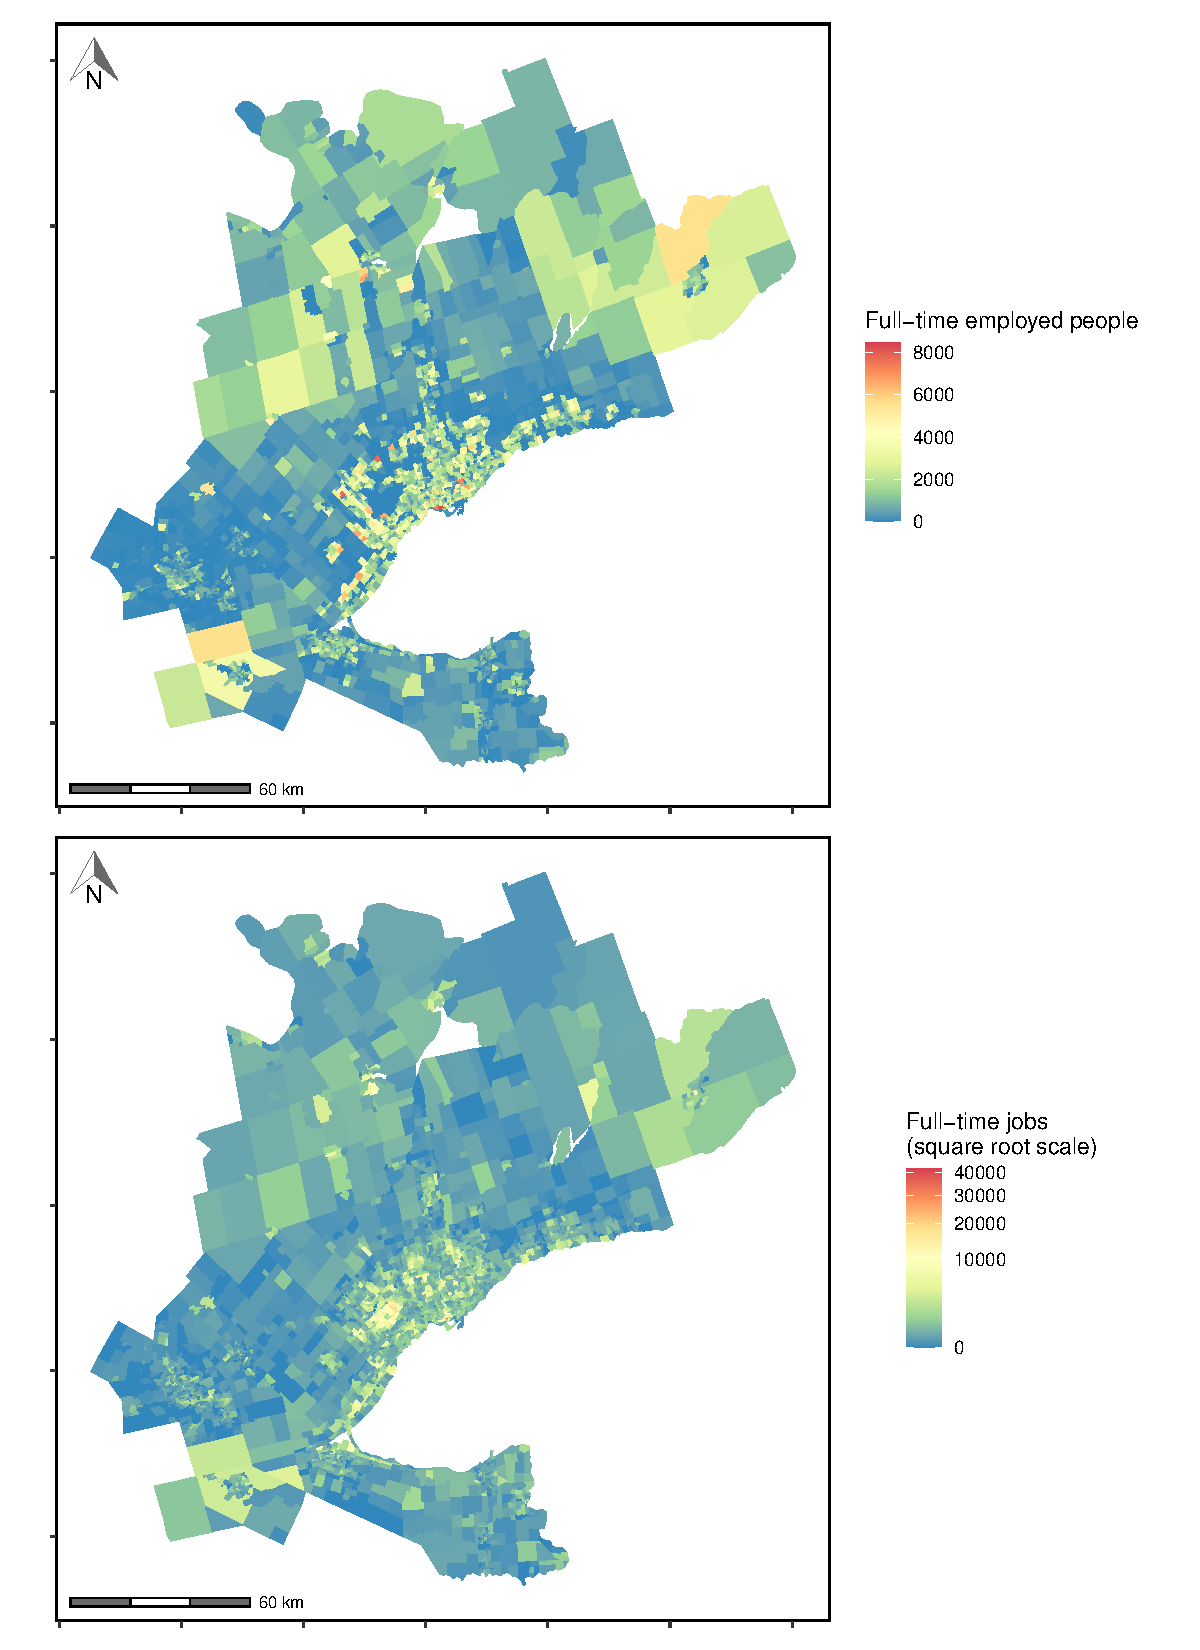
\includegraphics[width=1\linewidth]{Manuscript-Data-Package_files/figure-latex/tts-workers-jobs-plot-1} \caption{\label{fig:tts-workers-jobs-plot}Number of workers (top) and jobs (bottom) in each TAZ in the GGH area as specified by the 2016 TTS data set.}\label{fig:tts-workers-jobs-plot}
\end{figure}

\begin{figure}
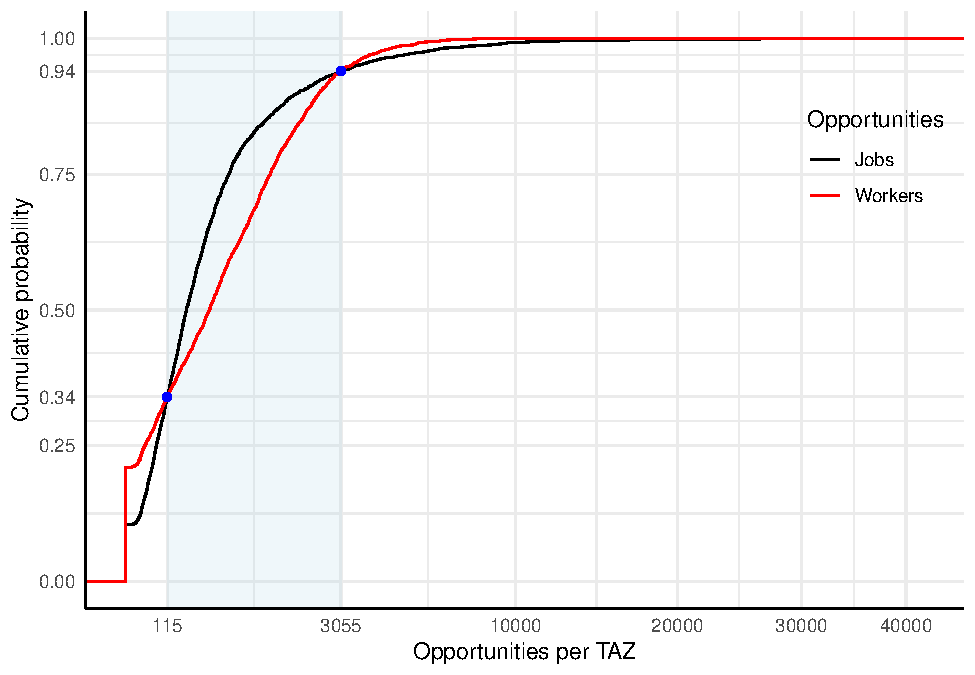
\includegraphics[width=1\linewidth]{Manuscript-Data-Package_files/figure-latex/ECD-plot-1} \caption{\label{fig:ECD-plot}The cumulative distribution of the number of jobs and workers per TAZ from the 2016 TTS data set. Light blue shaded ranges correspond to all cumulative proabilities where the number of workers per TAZ are larger than jobs per TAZ. }\label{fig:ECD-plot}
\end{figure}

Figure \ref{fig:tts-workers-jobs-plot} presents the number of workers
and jobs per TAZ. It can be observed that the spatial distribution of
jobs and workers is clearly not equal. Workers are concentrated in TAZ
within the center of the GGH and along the south-east and northern
boarder of the GGH. The center of the GGH corresponds to the Greater
Toronto Area (GTA) which is the most densely populated area in southern
Ontario \citep{statistics_canada_daily_2022}. The south east border of
the GGH neighbours Lake Ontario and is delineated by the urban built
boundary of the Ontario Growth Plan being home to the highest density of
working population in the GGH
\citep{ontario_built_2019, auditor_general_of_ontario_value_2021}. The
northern GGH border corresponds to the Simcoe, Dufferin, Kawartha Lake,
and Peterborough regions which are home to lower density of worker
population density population
\citep{auditor_general_of_ontario_value_2021}. Conversely, the spread of
jobs in the GGH is lower than the number of workers indicating employed
people are more spatially distributed than places of employment.

It can also be seen that from the bottom plot in Figure
\ref{fig:tts-workers-jobs-plot} that high to medium-low concentrations
of jobs are often present in the same areas as workers but only when the
scale is transformed. In other words, though there is a higher number of
TAZ with no workers than no jobs (i.e., 791 TAZ with no workers : 396
TAZ with no jobs) and the mean of workers per TAZ is higher than the
mean of jobs (i.e., 916 workers : 819 jobs) the number TAZ with an
extreme number of jobs at the highest and lowest percentiles is
significantly higher than the number of workers; see the following
cumulative probability distribution in Figure \ref{fig:ECD-plot} in
which the 94th to 100th percentile and the 0th to 34th percentile of
jobs in TAZ is higher than the number of workers in TAZ. This means that
between these ranges, TAZ have a higher number of workers than they do
jobs, echoing the more even spatial distribution of workers observed in
Figure \ref{fig:tts-workers-jobs-plot}.

\newpage

\hypertarget{calculated-travel-time}{%
\subsection{Calculated travel time}\label{calculated-travel-time}}

\texttt{AccessPack} also includes travel time data for each home-to-work
trip as displayed in Figure \ref{fig:plot-tt-ttpertrip}. This travel
time corresponds to a car commute calculated using the R package
\texttt{r5r} \citep{r5r_2021} and is interpreted as the travel time for
a work commute for full-time employed people in the GGH. The travel
times were calculated assuming the following input parameters: a 7:00 am
departure on Wednesday October 20th 2021, a maximum travel time less
than or equal to 180 mins (3 hrs), and a street network retrieved from
OpenStreetMaps for the GGH area. The 7:00 am departure corresponds to a
typical AM home-to-work departure and the 3 hr threshold was selected as
it captures 99\% of the trip taken (see the travel times summarized in
Table \ref{tab:TTS-16-desc-stats}).

It is important to note that all travel times within this data set are
calculated assuming car travel and one departure time for all origins.
These are unrealistic assumptions since we know a minority of trips are
taken by non-car modes and travel time departure varies, however, we do
not know which trips are made with non-car modes nor exact departures.
Though modal split and travel times can be estimated through other
methods \citep[e.g.,][]{allen_suburbanization_2021, higgins2021changes},
for simplicity, we carry on with the assumption that all trips are taken
by one-time departure car trip.

\begin{figure}
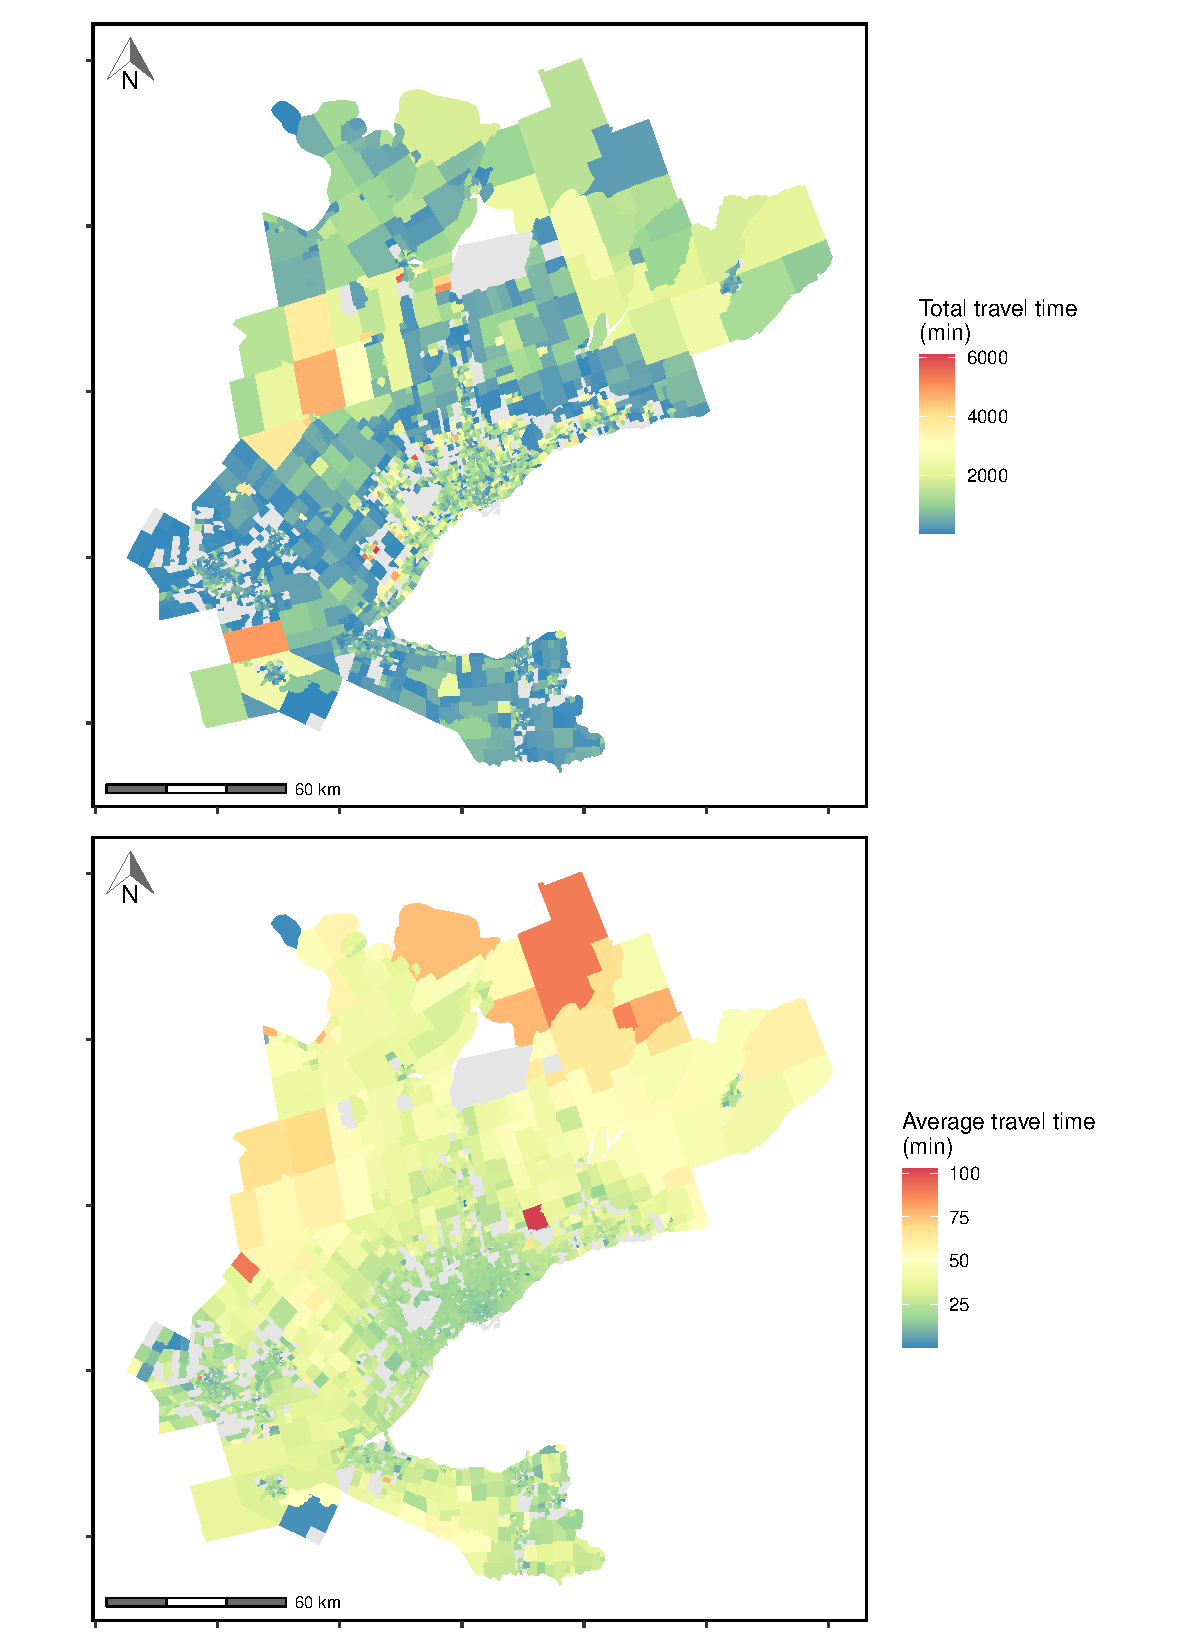
\includegraphics[width=1\linewidth]{Manuscript-Data-Package_files/figure-latex/plot-tt-ttpertrip-1} \caption{\label{fig:plot-tt-ttpertrip}Estimated total travel time (top) and average travel time per worker (bottom) for TAZ in the GGH.}\label{fig:plot-tt-ttpertrip}
\end{figure}

\newpage

As can be observed in Figure \ref{fig:plot-tt-ttpertrip}, the total
travel time (min) resembles the spatial trend distribution in the number
of employed people in the previous plot (Figure
\{fig:tts-workers-jobs-plot\}). However, when the average travel time
per trip in each TAZ is presented, the spatial distribution is distinct
from all other plots presented so far. We can see that in areas around
the south-eastern border that make up the Greater Toronto and Hamilton
Area (GTHA) (e.g., Hamilton, Halton, Peel, Toronto, York, Durham) and
Niagara and Waterloo, the average travel times are moderately low.
Further from these areas, travel times are higher. Interestingly, even
in eastern areas (e.g., Peterborough) with high employment and high job
concentration, average travel time is higher than within the GTHA.

\hypertarget{travel-cost-calibrating-an-impedance-function-for-accessibility}{%
\subsection{Travel cost: calibrating an impedance function for
accessibility}\label{travel-cost-calibrating-an-impedance-function-for-accessibility}}

With travel time and places of full-time employment,
\emph{accessibility} can be calculated. Accessibility is a measured
property of the origin (i.e., origin TAZ in our data) and is a common
approach to quantify the intensity of the potential for demand (i.e.,
workers) to interact with opportunities (i.e., jobs) . In other words,
accessibility in our case informs readers on how much full-time job
access each origin has for the people who reside there assuming travel
cost corresponds to the calibrated impedance function and the number of
full-time jobs. A widely used accessibility measure is based on the
gravity model and follows the formulation shown in Equation
(\ref{eq:conventional-accessibility}).

\begin{equation}
\label{eq:conventional-accessibility}
A_i = \sum_{j=1}^JO_jf(c_{ij})
\end{equation}

\noindent where:

\begin{itemize}
\tightlist
\item
  \(A\) is accessibility.
\item
  \(i\) is a set of origin locations.
\item
  \(j\) is a set of destination locations.
\item
  \(O_j\) is the number of opportunities at location \(j\). These are
  opportunities for activity and add some sort of \emph{supply} to the
  area;
\item
  \(c_{ij}\) is a measure of the cost of moving between \(i\) and \(j\)
\item
  \(f(\cdot)\) is an impedance function of \(c_{ij}\); it can take the
  form of any monotonically decreasing function chosen based on positive
  or normative criteria \citep{paez2012measuring}.
\end{itemize}

Formally, accessibility \(A_i\) is the weighted sum of opportunities
that can be reached from location \(i\), given the cost of travel
\(c_{ij}\). Summing the opportunities in the neighborhood of \(i\) as
defined by the impedance function \(f(\cdot)\), provides estimates of
the number of opportunities that can be reached from \(i\) at a certain
cost. This impedance function is often calibrated using the trip length
distribution (TLD) of the origin-destination data
\citep{horbachov_theoretical_2018, batista_estimation_2019} and the TLD
is the representation of the likelihood that a proportion of trips are
taken at a specific travel cost. In other words, in our data set where
we assume travel cost is travel time, a origin-destination trip with a
low travel time has a high impedance function value and a trip with a
high travel time has a low impedance function.

In the GGH data presented, the empirical TLD (i.e., proportion of trips
taken vs.~travel time in minutes) is fitted to a density distribution
using the maximum likelihood estimation and the Nelder-Mead method for
direct optimization available within the \texttt{fitdistrplus} package
\citep{fitdistrplus_2015}. Based on goodness-of-fit criteria and
diagnostics seen in Figure \ref{fig:TLD-Gamma-plot}, the gamma
distribution is selected for the presented data (also see Figure
\ref{fig:plot-cullen-frey} in the Appendix).

\begin{figure}
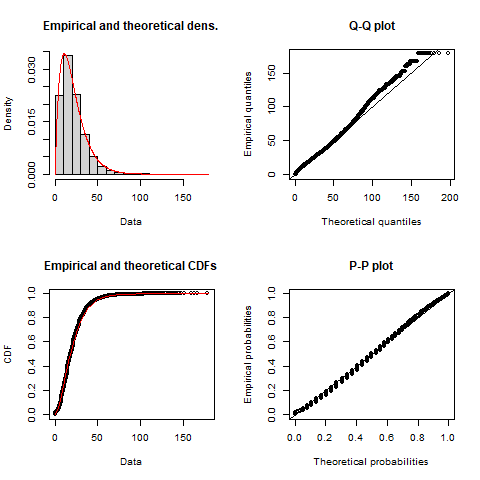
\includegraphics[width=1\linewidth]{images/impedance_function} \caption{\label{fig:TLD-Gamma-plot}Empirical TTS 2016 home-based car trip length distribution (black) and calibrated gamma distribution impedance function (red) with associated Q-Q and P-P plots}\label{fig:TLD-Gamma-plot}
\end{figure}

The resulting calibrated impedance function is given in the following
general form where the estimated `shape' is \(\alpha\) = 2.019, the
estimated `rate' is \(\beta\) = 0.094 , and \(\Gamma(\alpha)\) is
defined in Equation (\ref{gamma-dist}).

\begin{equation}
\label{gamma-dist}
\begin{array}{l}\ 
f(x, \alpha, \beta) = \frac {x^{\alpha-1}e^{-\frac{x}{\beta}}}{ \beta^{\alpha}\Gamma(\alpha)} \quad \text{for } 0 \leq x \leq \infty\\
\Gamma(\alpha) =  \int_{0}^{\infty} x^{\alpha-1}e^{-x} \,dx\\
\end{array}
\end{equation}

\hypertarget{calculating-job-access-in-different-ways}{%
\section{Calculating job access in different
ways}\label{calculating-job-access-in-different-ways}}

As introduced in Equation (\ref{eq:conventional-accessibility}),
accessibility can be simply calculated for the origins in each TAZ. The
accessibility value for each TAZ represents how many opportunities,
after being discounted by their travel cost, are \emph{potentially}
accessible to the population within that TAZ. There have been many types
of accessibility equations proposed and the field of research is
continuously growing so developing an easy-to-manipulate
empirically-based data set, as presented in this paper, is essential to
experimenting with novel iterations of measures.

For instance, in \texttt{AccessPack}, a function for a newly proposed
\emph{singly-constrained competitive} accessibility measure referred to
as spatial availability is available to use. This new measure responds
to the criticism that the conventional accessibility measure is not
explicitly meaningful \citep{miller2018} and does not consider
competition \citep{luo2003}. It seeks to answer the following questions
which the conventional accessibility measure Equation
(\ref{eq:conventional-accessibility}) can not :

\begin{itemize}
\tightlist
\item
  ``many opportunities are accessible, but the same opportunities are
  also accessible to my (possibly) numerous neighbours\ldots{} what does
  a high accessibility actually mean to me?''; and
\item
  ``a few opportunities are accessible to me but I am located in a
  remote area with proportionally few neighbours relative to the
  region\ldots{} what does low accessibility mean to me?''.
\end{itemize}

The proposed spatial availability measure proportionally allocates the
number of opportunities based on the travel cost and demand population
(i.e., workers) constraints the number of opportunities and is presented
in it's general form in Equation \ref{eq:spatial-availability}. Please
see the forthcoming
\href{https://github.com/soukhova/Spatial-Availability-Measure}{article}
for an in-depth introduction and discussion on how it differs from the
conventional accessibility measure.

\begin{equation}
\label{eq:spatial-availability}
V_{ij} = O_j\frac{F^p_{ij} \cdot F^c_{ij}}{\sum_{i=1}^K F^p_{ij} \cdot F^c_{ij}}
\end{equation}

\noindent where:

\begin{itemize}
\tightlist
\item
  \(V_{ij}\) is spatial availability.
\item
  \(i\) is a set of origin locations in the region \(K\).
\item
  \(j\) is a set of destination locations in the region \(K\).
\item
  \(O_j\) is the number of opportunities at location \(j\) in the region
  \(K\).
\item
  \(F^p_{ij}\) is the proportional allocation factor of the population
  in \(i\) relative to the population in region \(K\).
\item
  \(F^c_{ij}\) is the proportion allocation factor of travel cost for
  \(i\) relative to the travel cost in region \(K\); it is a product of
  a monotonically decreasing (i.e., impedance) function associated with
  the cost of travel between \(i\) and \(j\).
\end{itemize}

Figure \ref{fig:plot-access-SA-GGH-TTS} visualizes the two opportunity
access measures which can facilitate understanding on how the measures
differ. The accessibility plot follows a distinct radial trend where the
majority of TAZ in Toronto have high accessibility values and values
gradually decrease in TAZ which are further from Toronto's boundary
(show in grey outline). Conversely, spatial availability does not appear
to follow a radial trend and values appear more even throughout the GGH
in comparison to job access as measured by accessibility. This can be
noted in higher values around the north east and south west periphery
TAZ and more moderate values in and around Toronto.

\begin{figure}
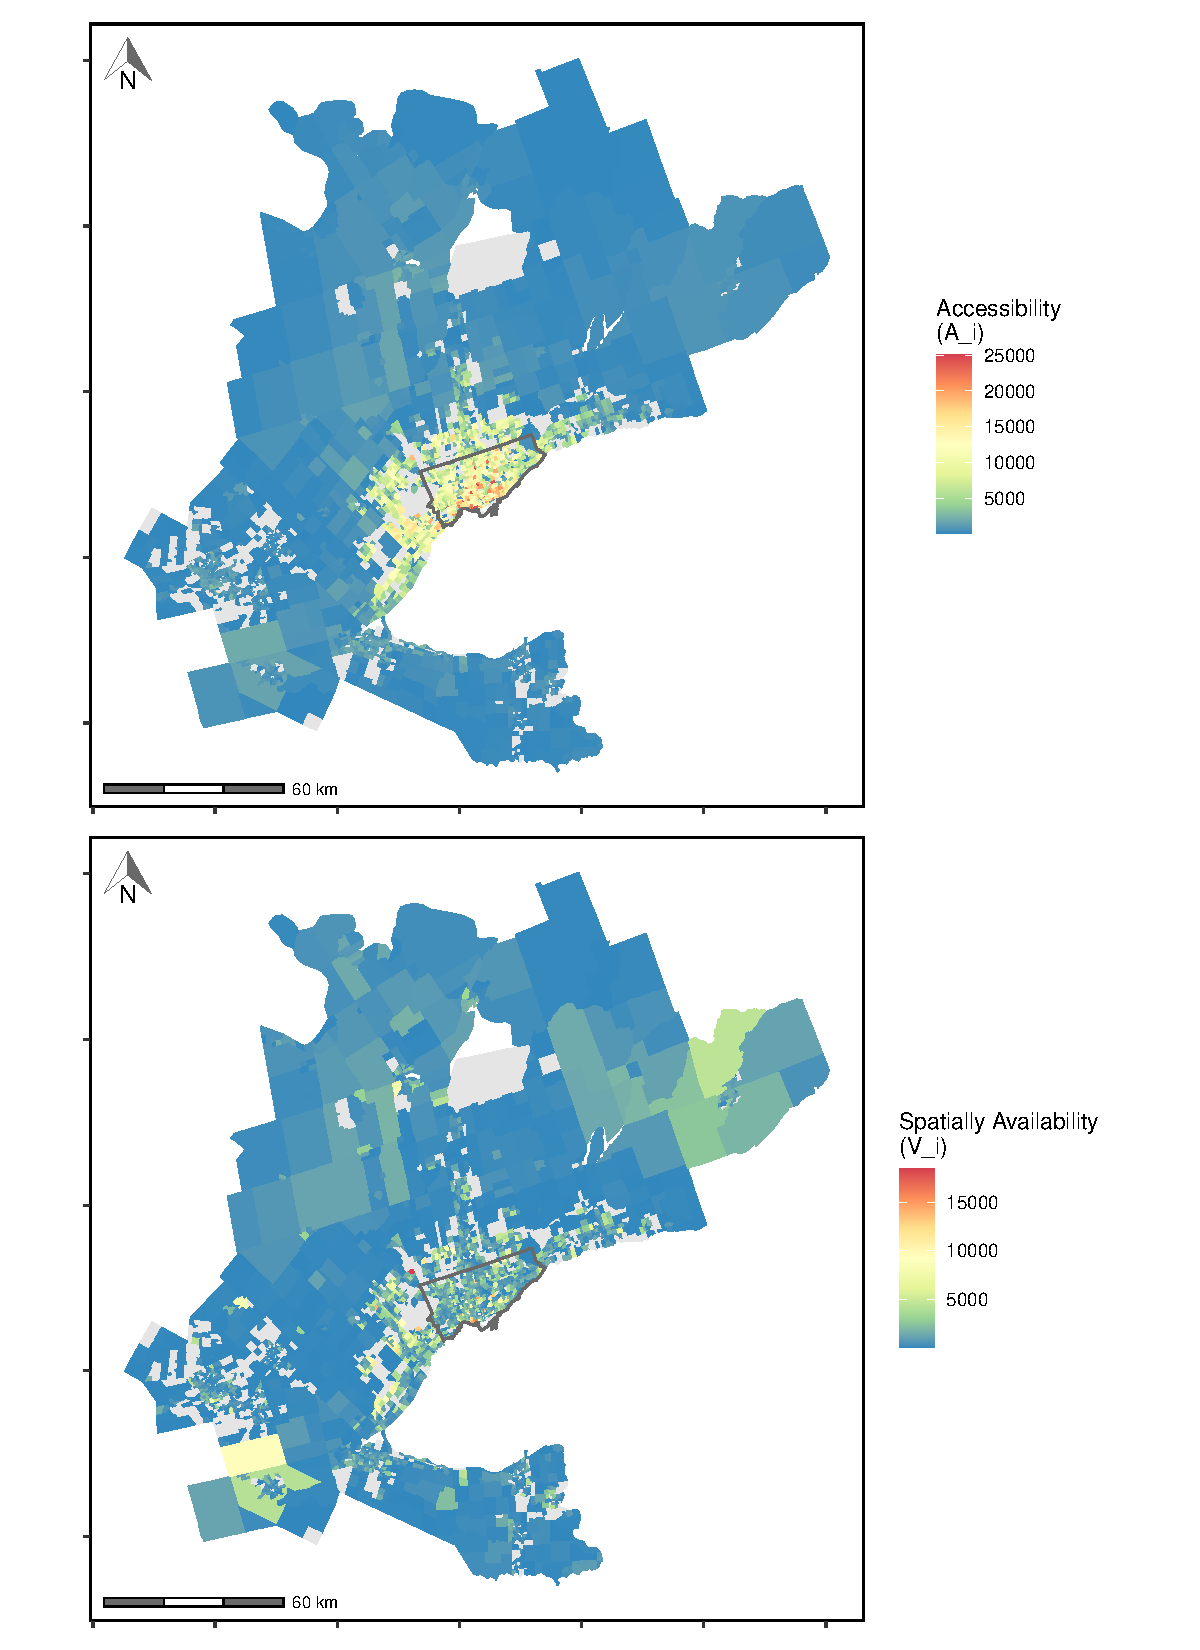
\includegraphics[width=1\linewidth]{Manuscript-Data-Package_files/figure-latex/plot-access-SA-GGH-TTS-1} \caption{\label{fig:plot-access-SA-GGH-TTS}Calculated accessibility (top) and spatial availability (bottom) of employment in the GGH area}\label{fig:plot-access-SA-GGH-TTS}
\end{figure}

\newpage

Alternatively, Figure \ref{fig:plot-avail-GGH-TTS-per-worker} presents
spatial availability normalized by worker in which pinkish-red is above
average job access, blueish is below average job access, and white is
average job access (i.e., 0.89 jobs per worker). The trends seen in the
spatial availability plot in the previous plot (Figure
\ref{fig:plot-access-SA-GGH-TTS}) are identical, however, normalizing
the access value by simply dividing the spatial availability value for
each TAZ by the worker population in that TAZ results in a meaningful
job access landscape. It should be noted, that since opportunities are
\emph{proportionally} allocated to each origin, the total sum of job
access is equal to the total sum of jobs. So, the average spatial
availability of 0.89 jobs per worker means each full-time worker in a
TAZ with average spatial availability have access to 0.89 jobs.

\begin{figure}
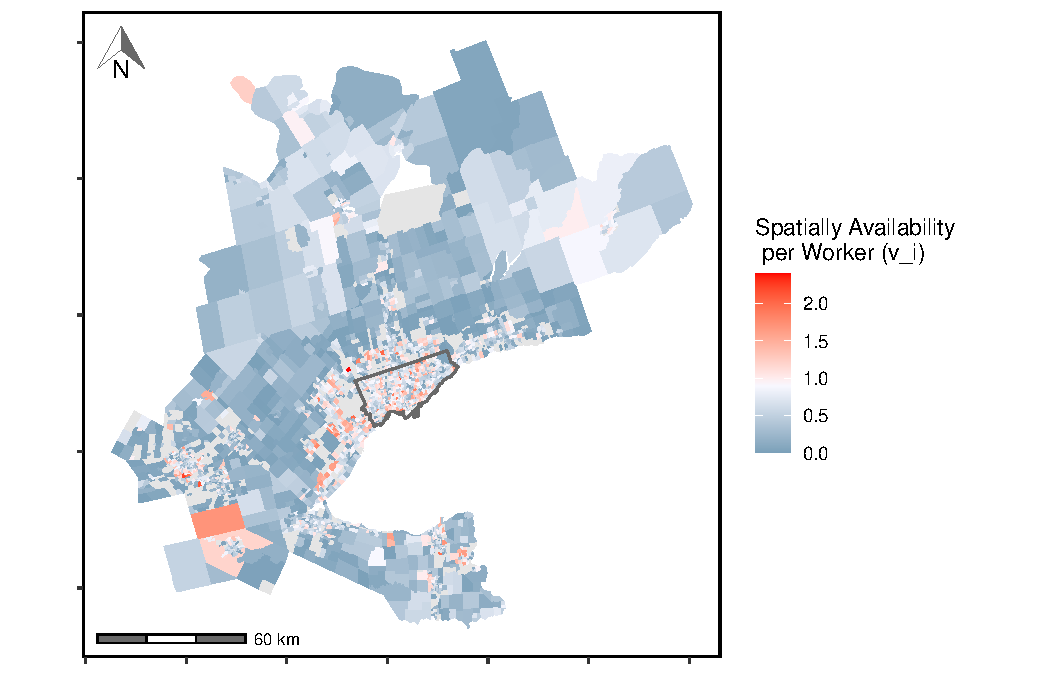
\includegraphics[width=1\linewidth]{Manuscript-Data-Package_files/figure-latex/plot-avail-GGH-TTS-per-worker-1} \caption{\label{fig:plot-avail-GGH-TTS-per-worker}Calculated spatial availability of employment, per worker, from origins to destinations in the GGH.}\label{fig:plot-avail-GGH-TTS-per-worker}
\end{figure}

\newpage

\hypertarget{concluding-remarks}{%
\section{Concluding remarks}\label{concluding-remarks}}

This paper showcases the home-to-work data from the 2016 TTS and how it
was used to calculate job access in southern Ontario, Canada using two
types of accessibility measures. The data and the new opportunity access
measure, \emph{spatial availability} , are both packaged in the open
data product
\href{https://github.com/soukhova/AccessPack}{\texttt{AccessPack}} which
can be explored in an R environment. The proposed spatial availability
is a singly-constrained competitive measure discussed in detailed within
a forthcoming
\href{https://github.com/soukhova/Spatial-Availability-Measure}{article}.

New digital formats are increasingly complex and the explanation of the
methods often do not concisely and intelligibly fit within the confines
of a traditional article. With this motivation, we invite all who are
interested to explore \texttt{AccessPack} and respond to the differences
between conventional gravity-based accessibility measures, our newly
proposed measure, or simply manipulate and visualize the empirical data
presented in the package. In the spirit of novel and original research,
we hope readers value the efforts made to detail the data and methods in
greater depths in order to improve transparency in our work and
encourage others to replicate and, hopefully, propose better and
different methods.

\hypertarget{appendix}{%
\section{Appendix}\label{appendix}}

\begin{figure}
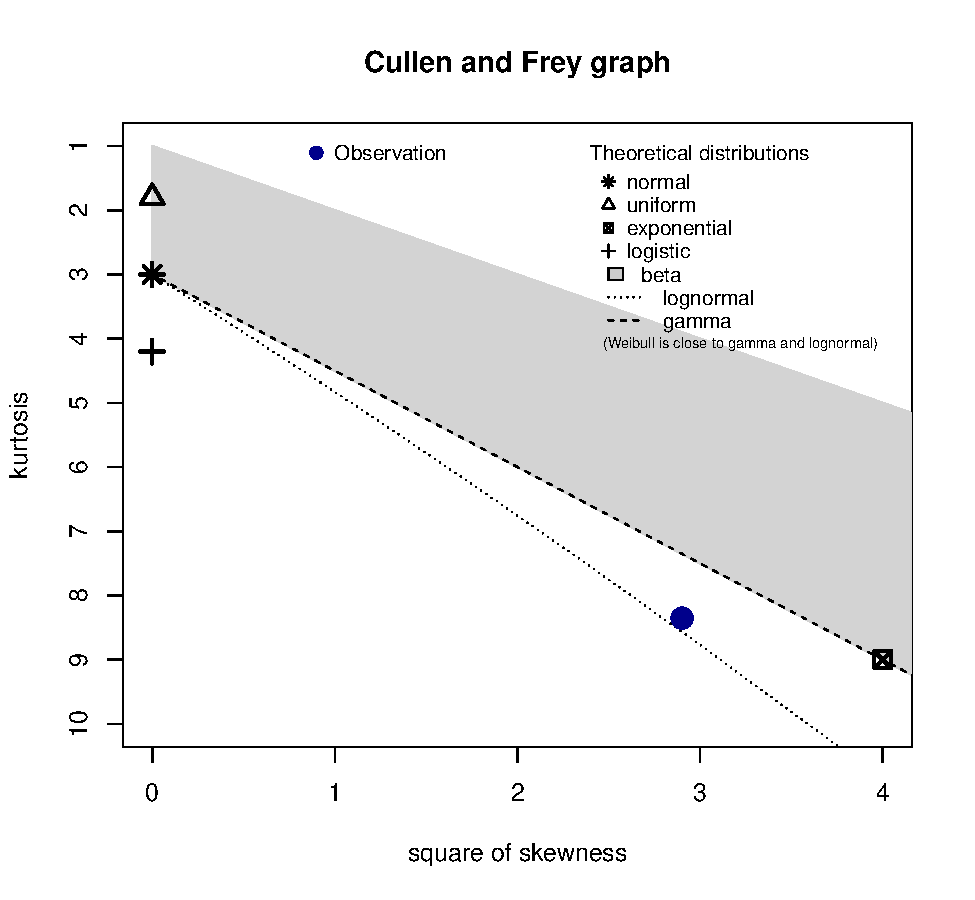
\includegraphics[width=1\linewidth]{Manuscript-Data-Package_files/figure-latex/plot-cullen-frey-1} \caption{\label{fig:plot-cullen-frey}Cullen and frey graphy for the 2016 TTS calculated travel times.}\label{fig:plot-cullen-frey}
\end{figure}

\begin{verbatim}
summary statistics
------
min:  0.1   max:  179 
median:  18 
mean:  21.4344 
estimated sd:  14.61254 
estimated skewness:  1.703326 
estimated kurtosis:  8.353363 
\end{verbatim}

\newpage

\bibliographystyle{sageh}
\bibliography{bibfile}


\end{document}
